
\begin{figure}[ht]
\begin{Verbatim}[numbers=right,fontsize=\codesize,commandchars=\*\{\}]
type left(node, node).*label{line:language:dict_header1}
type right(node, node).
type linear value(node, int Key, string Value).
type linear replace(node, int Key, string Value).*label{line:language:dict_header2}

replace(A, K, New),*label{line:language:dict_first1}
value(A, K, Old)
   -o value(A, K, New). // we found our key*label{line:language:dict_first2}

replace(A, RKey, RValue),*label{line:language:dict_second1}
value(A, Key, Value),
!left(A, B),
RKey < Key
   -o value(A, Key, Value),
      replace(B, RKey, RValue). // go left*label{line:language:dict_second2}

replace(A, RKey, RValue),*label{line:language:dict_third1}
value(A, Key, Value),
!right(A, B),
RKey > Key
   -o value(A, Key, Value),
      replace(B, RKey, RValue). // go right*label{line:language:dict_third2}

// initial configuration*label{line:language:dict_axioms1}
!left(@0, @1).     !right(@0, @2).
!left(@1, @3).     !right(@1, @4). 
!left(@2, @5).     !right(@2, @6).

value(@0, 3, "a").   value(@1, 1, "b").
value(@2, 5, "c").   value(@3, 0, "d").
value(@4, 2, "e").   value(@5, 4, "f").
value(@6, 6, "g").

// update key 6 to value "x"
replace(@0, 6, "x").*label{line:language:dict_axioms2}
\end{Verbatim}
\caption{LM program for replacing a key's value in a BST dictionary.}
\label{code:btree_replace}
\end{figure}

Our first example, shown in Fig.~\ref{code:btree_replace}, implements the key
update operation for a binary tree search~(BST) represented as a key/value
dictionary. Each LM node represents a binary tree node. We first declare all the
predicates
(lines~\ref{line:language:dict_header1}-\ref{line:language:dict_header2}), which
represent the kinds of facts we are going to use. Note that the first argument
of every predicate must be typed as \texttt{node} because the first argument
indicates where the node lives in the graph. Predicates \texttt{left/2} and
\texttt{right/2} are persistent while \texttt{value/3} and \texttt{replace/3}
are linear. Persistent predicates are preceded with a \texttt{!} symbol in LM
rules for improved readability. Linear predicate \texttt{value/3} assigns a
key/value pair to a node that can be updated later.  The \texttt{replace/3}
linear predicate represents an update operation where the key in the second
argument will be updated to the value in the third argument.

The algorithm uses three rules for the three possible cases of updating a key's
value: the first rule
(lines~\ref{line:language:dict_first1}-\ref{line:language:dict_first2}) performs
the update by removing \texttt{replace(A, K, New)} and \texttt{value(A, K, Old)}
and deriving \texttt{value(A, K, New)}; the second rule
(lines~\ref{line:language:dict_second1}-\ref{line:language:dict_second2})
recursively picks the left branch for the update operation by deleting
\texttt{replace(A, RKey, RValue)} and re-deriving it at node \texttt{B}; and the
third rule
(lines~\ref{line:language:dict_third1}-\ref{line:language:dict_third2}) picks
the right branch. Note that in all the rules, the body of each rule uses facts
from the same node (in this particular case, \texttt{A}), but the head of the
rule may derive facts in other nodes (e.g., the second and third rules) because
a node variable was instantiated in the body of the rule. Moreover, persistent
facts used in the body of the rule are not deleted after rule application - only
linear facts are. The axioms of this program are presented in
lines~\ref{line:language:dict_axioms1}-\ref{line:language:dict_axioms2} and they
describe the initial binary tree configuration, including keys and values.  The
axiom \texttt{update(@0, 6, "x")} instantiated at the root node \texttt{@3}
manifests the intent to change the value of key 6 to 7.

Fig.~\ref{fig:btree_trace} represents the trace of the algorithm. The program
database is partitioned by the seven nodes using the first argument of each
fact. In Fig.~\ref{fig:btree_trace}~(a), we present the database filled with the
program's axioms. Next, we follow the right branch using rule 3 since $6 > 3$
(Fig.~\ref{fig:btree_trace}~(b)).  We use the same rule again in
Fig.~\ref{fig:btree_trace}~(c) where we finally reach the key 6. Here, we apply
rule 1 and \texttt{value(@6, 6, "g")} is updated to \texttt{value(@6, 6, "x")}.

\begin{figure}[h]
        \centering
        \begin{subfigure}[b]{0.5\textwidth}
                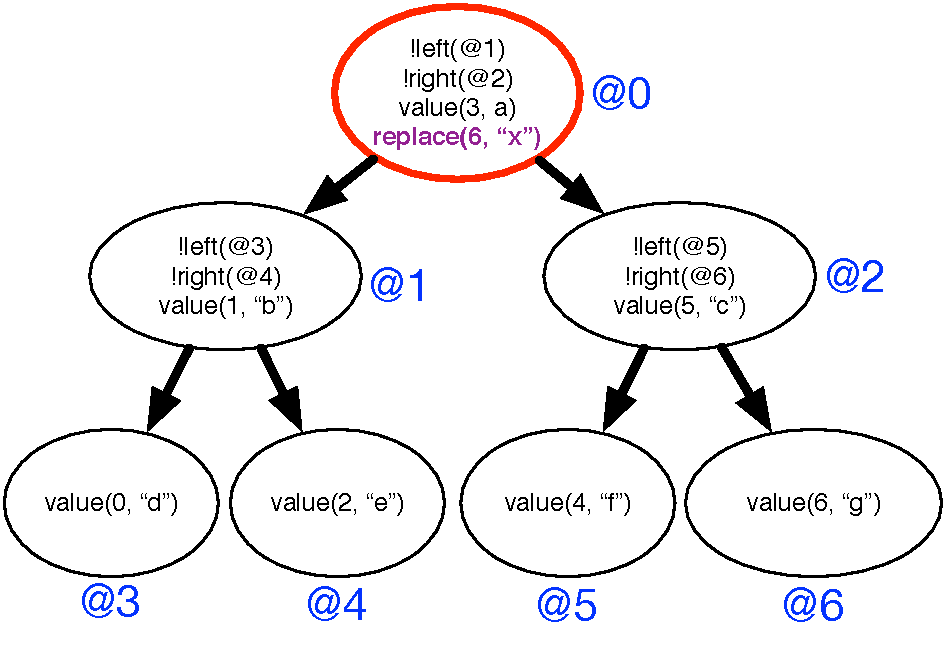
\includegraphics[width=\textwidth]{figures/btree/btree_trace1}
                \caption{Initial database. Replace axiom instantiated at the
                   \texttt{@3} root node.}
                \label{fig:btree_trace1}
        \end{subfigure}%
        ~
        \begin{subfigure}[b]{0.5\textwidth}
                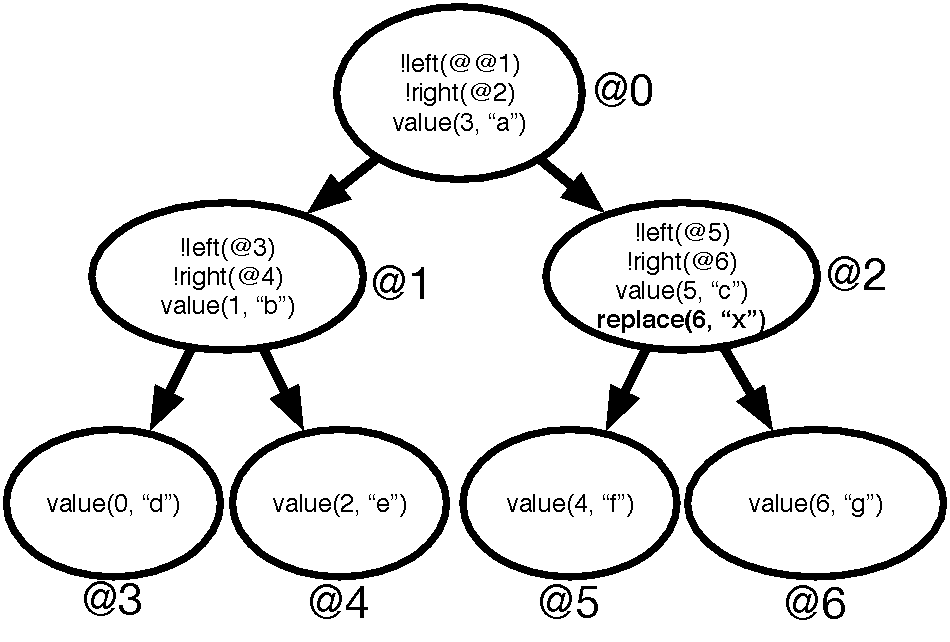
\includegraphics[width=\textwidth]{figures/btree/btree_trace2}
                \caption{After applying rule 3 at node \texttt{@3}. Replace fact
                   sent to node \texttt{@5}.}
                \label{fig:btree_trace2}
        \end{subfigure}\\
        \begin{subfigure}[b]{0.5\textwidth}
                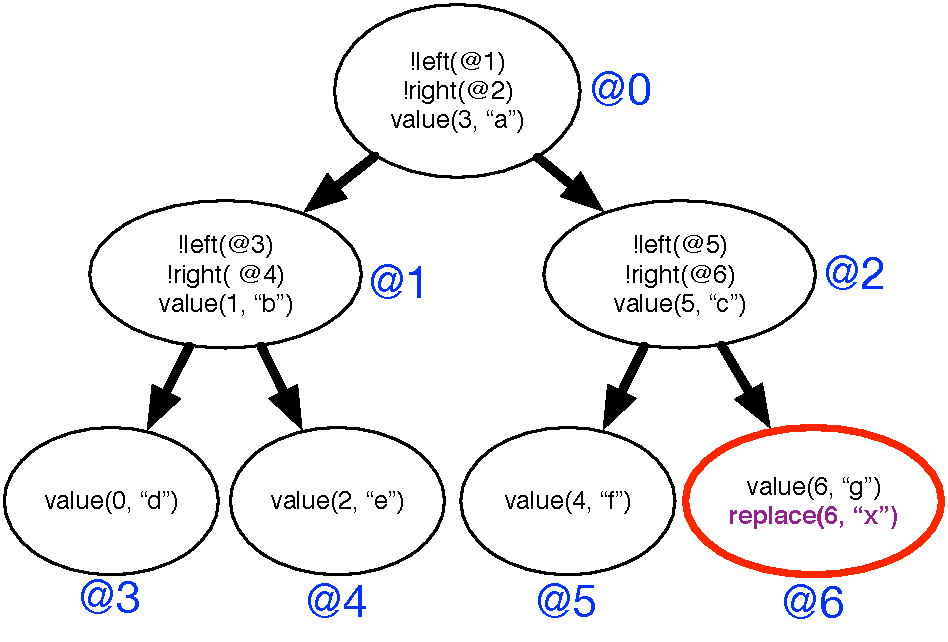
\includegraphics[width=\textwidth]{figures/btree/btree_trace3}
                \caption{After applying rule 3 at node \texttt{@5}. Replace fact
                   reaches node \texttt{@6}.}
                \label{fig:btree_trace3}
        \end{subfigure}%
        ~
        \begin{subfigure}[b]{0.5\textwidth}
                  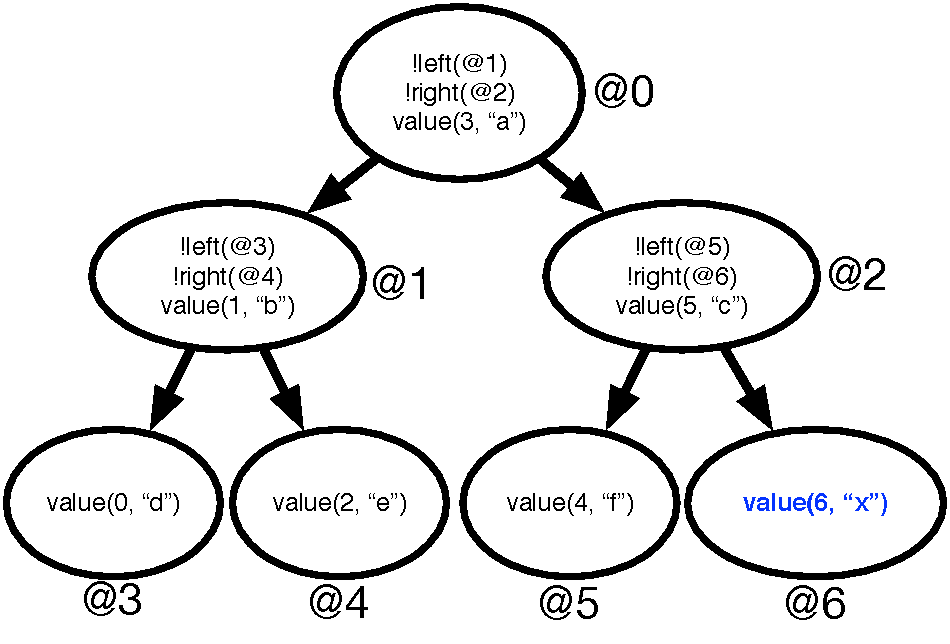
\includegraphics[width=\textwidth]{figures/btree/btree_trace4}
                  \caption{After applying rule 1 at node \texttt{@6}. Value of key 6 has changed to 7.}
                  \label{fig:btree_trace4}
          \end{subfigure}
        \caption{An execution trace for the binary tree dictionary
           algorithm. The first argument of each fact was dropped and the
           address of the node was placed beside it.}\label{fig:btree_trace}
\end{figure}

The present example offers many opportunies for concurrency. If we have multiple
\texttt{replace/3} facts on different nodes, we can perform multiple value
updates at the same time without introducing any kind of database inconsistency.

